\documentclass[a4paper,12pt]{article}
\usepackage[utf8]{inputenc}
\usepackage[czech]{babel}
\usepackage[T1]{fontenc}
\usepackage{geometry}
\geometry{a4paper, margin=2cm}
\usepackage{graphicx}
\usepackage{hyperref}
\usepackage{booktabs}
\usepackage{float}
\usepackage{fancyhdr}

\setlength{\headheight}{1.5cm}
\pagestyle{fancy}
\fancyhf{}
\renewcommand{\headrulewidth}{0.4pt}

% Záhlaví vlevo: Hydra logo
\fancyhead[L]{
\includegraphics[height=1.2cm]{hydra.png}}

% Záhlaví vpravo: Text vertikálně zarovnaný vedle HSP loga
\fancyhead[R]{
    \raisebox{0.4cm}{\textbf{Draft finálového reportu}}\hspace{0.3cm}
    
\includegraphics[height=1.2cm]{hsp_logo.png}
}

% Zápatí: číslo stránky uprostřed
\fancyfoot[C]{\thepage}

\begin{document}

\begin{titlepage}
    \centering
    \vspace*{2cm}
    
\includegraphics[width=10cm]{hsp_logo.png}\\[2cm]
    
    {\Huge \textbf{Draft finálového reportu}\par}
    \vspace{1cm}
    {\Huge \textbf{Tým Hydra}\par}
    \vspace{1.5cm}
    {\Large \textbf{Kategorie:} Začátečníci SŠ\par}
    
    \vfill
    {\Large \today\par}
\end{titlepage}

\section{Úvod}
Jsme tým \textbf{Hydra} a předkládáme tento finálový report do kategorie Začátečníci SŠ v rámci Czech Rocket Challenge. 
V tomto dokumentu detailně popisujeme návrh, výrobu a simulaci naší rakety, včetně použitých palubních systémů a plánovaných testů.

\section{Tabulka parametrů}
% Kategorie, Apogeum, Délka, Průměr, Hmotnost, Stabilita, Akcelerace, Doba letu, Rychlost sestupu.
\begin{table}[H]
    \centering
    \begin{tabular}{lc}
        \toprule
        \textbf{Parametr} & \textbf{Hodnota} \\
        \midrule
        Kategorie & Začátečníci SŠ \\
        Předpokládané apogeum & 558 m \\
        Délka rakety & 550 mm \\
        Průměr trupu & 63 mm \\
        Očekávaná hmotnost bez motoru & 897 g \\
        Stabilita při opuštění rampy & 1.05 cal. \\
        Stabilita maximální & 1.73 cal. \\
        Maximální akcelerace & 101.6 m$\cdot$s$^{-2}$ \\
        Doba letu & 91.9 s \\
        Rychlost sestupu & 8.0 m$\cdot$s$^{-1}$ \\
        \bottomrule
    \end{tabular}
    \caption{Základní parametry rakety}
\end{table}

\section{Struktura rakety}
Hlavní trup rakety tvoří hotová uhlíková (carbonová) trubka od výrobce OXXO, což zajišťuje maximální pevnost při zachování nízké hmotnosti. Přední špička (nose cone) je vyrobena metodou 3D tisku z materiálu ASA a následně vyhlazena parami acetonu pro dosažení optimálních aerodynamických vlastností a mechanické odolnosti. Přepážky v raketě jsou tištěny z materiálu ABS.

Výroba a montáž probíhá následovně: Stabilizátory rakety jsou vyřezány CNC strojem z uhlíkových plátů (ve spolupráci se SITPortem v Plzni). Následně jsou stabilizátory zasunuty až dovnitř trupu a přilaminovány k němu. Pro maximální zpevnění je mezi každými dvěma sousedními stabilizátory navíc přelaminována skelná tkanina. Samotný raketový motor se šroubuje do vlastního lože, zasouvá se mezi vnitřní části stabilizátorů a celý systém se zvenku upevní a zajistí přišroubováním vnější klapky.

\section{OpenRocket simulace}
Simulace chování rakety probíhala v softwaru OpenRocket. V návrhu byly pečlivě specifikovány jednotlivé díly a parametry letu pro ověření bezpečné stability a letových vlastností.

\begin{figure}[H]
    \centering
    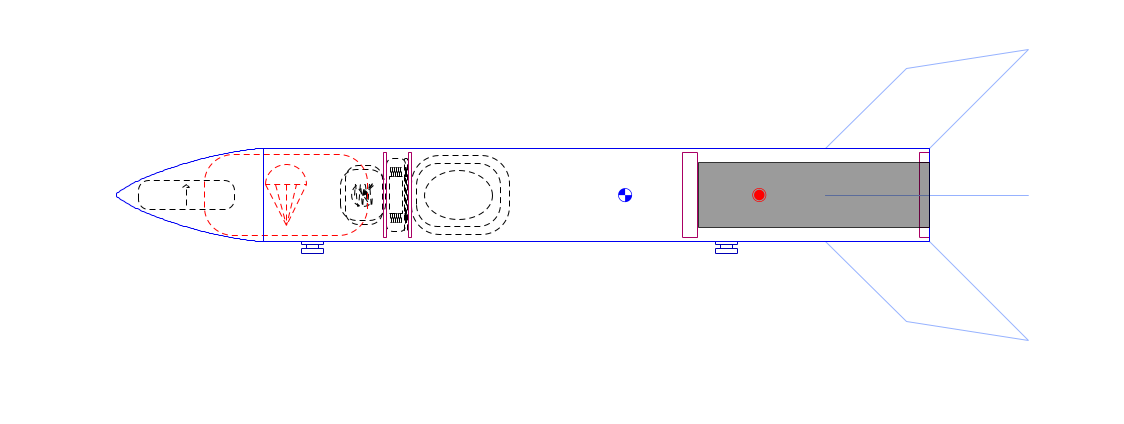
\includegraphics[width=0.8\textwidth]{img/design_rakety.png}
    \caption{Návrh rakety v OpenRocket s pojmenovanými komponentami}
\end{figure}

\begin{figure}[H]
    \centering
    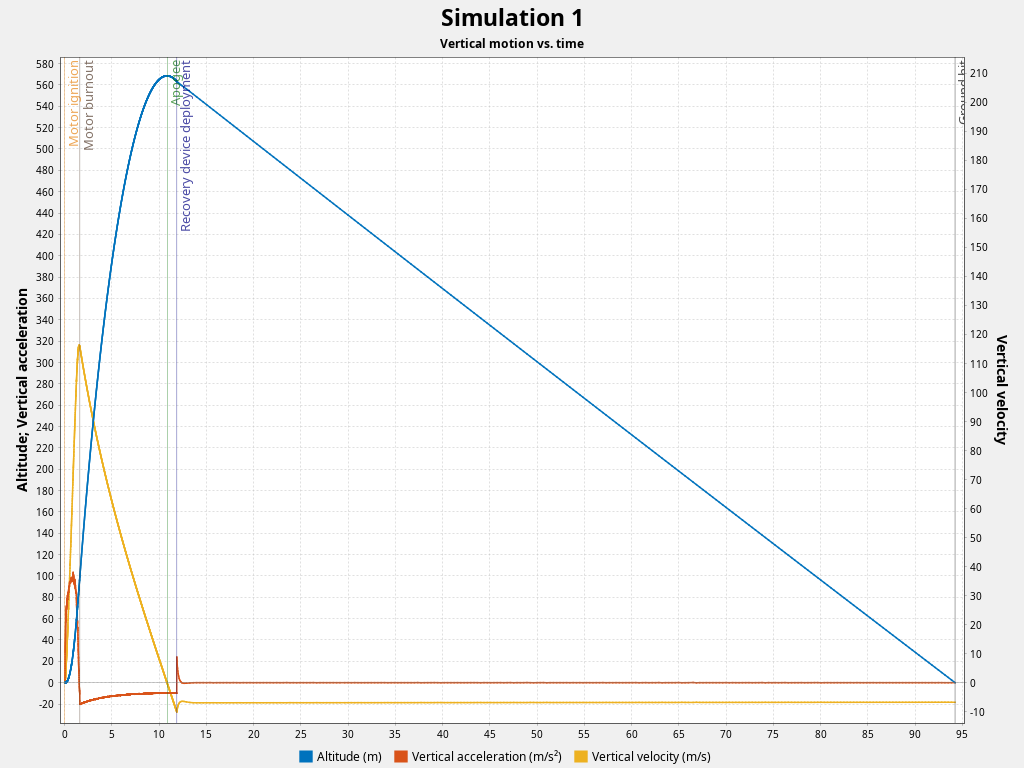
\includegraphics[width=0.8\textwidth]{img/VerticalMotion_x_Time.png}
    \caption{Graf letové simulace (vertikální pohyb v čase)}
\end{figure}

\begin{figure}[H]
    \centering
    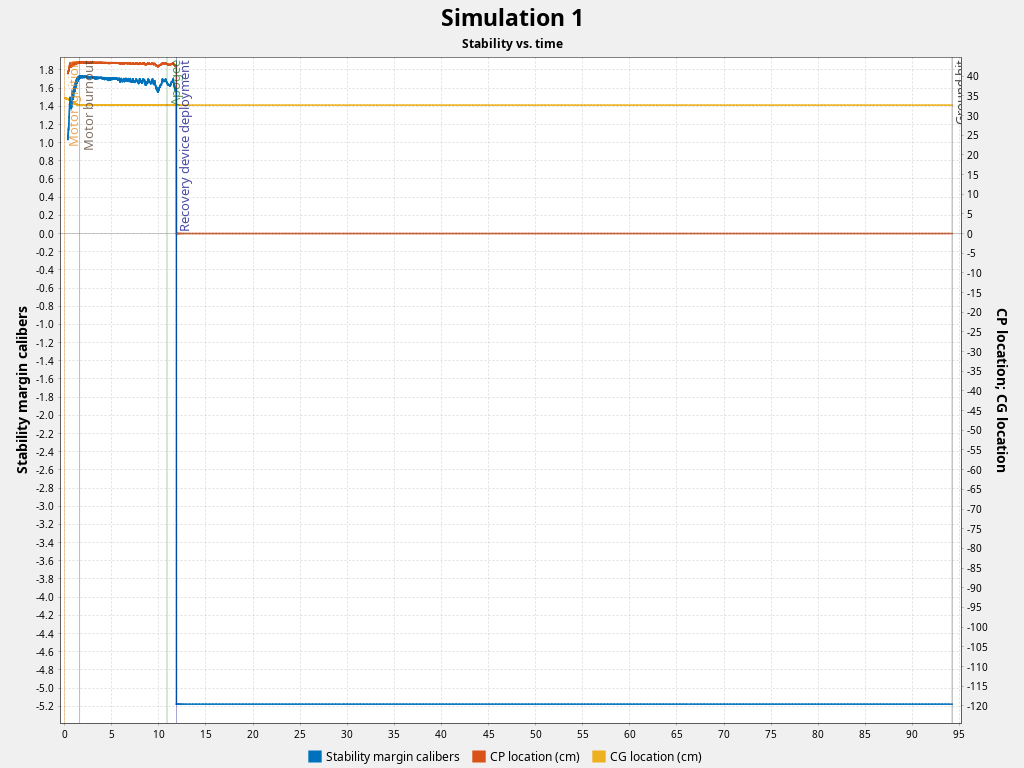
\includegraphics[width=0.8\textwidth]{img/Stability_x_Time.png}
    \caption{Graf vývoje stability rakety v průběhu letu}
\end{figure}

\section{Záchranný systém}
Záchranný systém využívá k vypuštění padáku výmetnou nálož (ejection charge). Systém je navržen s důrazem na maximální bezpečnost a zálohování, a proto disponuje dvěma nezávislými řídícími obvody a dvěma palníky.

\textbf{Hlavní systém:}
Řízení obstarává mikrokontrolér Raspberry Pi Pico, který čte letová data a filtruje je pomocí Kalmanova filtru k přesné detekci okamžiku startu a dosažení apogea. V apogeu hlavní počítač odpálí první ze dvou palníků.

\textbf{Záložní systém:}
Jako záloha slouží nezávislý mikrokontrolér ATtiny402. Ten detekuje start čistě mechanicky pomocí přetržení odtrhového vodiče (breakaway wire). Po detekci startu se spustí časovač nastavený podle doby letu do apogea (z OpenRocket simulace) s přičtenou bezpečnostní časovou rezervou. Přidaná rezerva zajišťuje, že při standardním letu zasáhne vždy jako první hlavní systém. Pokud by ale selhal nebo došlo k nestandardnímu letu, odpočítávání garantuje nezávislé odpálení druhého palníku.

\section{Challenge}
V rámci splnění výzvy kategorie Začátečníci jsme navrhli speciální nárazuvzdorné pouzdro pro ochranu syrového vejce. Záchranný systém vejce tvoří dvě polystyrenové poloviny tvaru poloválce (rozpůlené vertikálně), ve kterých je vytvořen přesný otvor pro velikost vejce. 
Po vložení vejce se obě polystyrenové půlky zaklapnou k sobě a takto spojený celek se zasune do vnitřního prostoru trupu rakety. Díky těsnému uložení pouzdra v trupu se polystyrenové poloviny nemohou od sebe odpojit, což poskytuje vajíčku pevnou, jednoduchou a maximálně bezpečnou ochranu před poškozením při dopadu.

\section{Ejection charge}
Pro výmet padáku je použito 0.3~g střelného prachu odpalovaného elektrickým palníkem.
Z důvodu bezpečnosti na odpalovací rampě je raketa vybavena RBF (Remove Before Flight) pojistkou s velkou červenou stuhou. Zasunutím RBF pinu dojde ke stisknutí koncového přepínače, který rozpojí dva kontakty a tím fyzicky (elektricky) přeruší obvod k výmetné náloži. Při vytažení RBF pinu na rampě se obvod uzavře a palubní avionika potvrdí odjištění (armování) rakety dlouhým zřetelným tónem ze zabudovaného bzučáku.

\section{Pojezdy}
Finální podoba a materiál pojezdů (rail buttons) je v současnosti ještě ve fázi řešení a testování. Jako nejoptimálnější návrh se v tuto chvíli jeví využití dvojice pojezdů z odolného plastu Delrin o vnějším průměru 15~mm, které by měly být na trupu umístěny s rozestupem 280~mm. Zvolený tvar a materiál by zajistil hladký a bezpečný výstup po koleji s minimálním třením. Konkrétní řešení bude s konečnou platností potvrzeno před finálovým letem.

\section{Groundstation}
Telemetrie z rakety je přijímána přes přenosnou pozemní stanici. Tu tvoří mikrokontrolér z rodiny ESP (mini), ke kterému je připojen bezdrátový rádiový modul HC-12. Modul přijímá zprávy od identického HC-12 vysílače na palubě rakety a přes USB rozhraní přeposílá získaná data k vyhodnocení do připojeného počítače.

\section{Avionika}
Palubní elektronika je z důvodu modularity a přehlednosti rozdělena na tři samostatné desky:
\begin{itemize}
    \item \textbf{Napěťová deska:} Obsahuje obvody pro spínání palníků, čip rodiny INA pro měření napětí a proudu a akustický bzučák.
    \item \textbf{Logická deska:} Srdcem desky je Raspberry Pi Pico, které sbírá data ze senzorů -- barometru ICP-10101 od TDK Invensense a akcelerometru řady LSM6D.
    \item \textbf{GPS a Telemetrie:} Samostatná deska obsahující GPS modul u-blox SAM-M8Q a rádiový modul HC-12.
\end{itemize}

*(Functional flow diagram softwarových stavů bude doplněn v průběhu příprav.)*

\section{Výškoměr}
Funkci výškoměru plní barometr ICP-10101 integrovaný na logické desce. Pro správné snímání statického okolního tlaku byly na vnějším trupu navrženy a vyvrtány 3 symetricky rozmístěné otvory (od sebe $120^\circ$) o průměru 3~mm. Tyto porty zajišťují vyrovnávání tlaku bez negativního ovlivnění aerodynamickým obtékáním.

\section{Procedury}
Pro zajištění maximální bezpečnosti a hladkého průběhu startu jsme připravili krok-za-krokem checklist pro finálový den soutěže:

\subsection*{Příprava a kontrola na místě}
\begin{enumerate}
    \item Příchod týmu na místo konání a registrace.
    \item Přesun do přípravného depa a vybalení komponent rakety.
    \item Vizuální kontrola trupu, špičky, stabilizátorů a pojezdů po transportu.
    \item Kontrola pevných spojů a laminace trupu.
    \item Sestavení a kontrola mechanického pouzdra na vejce (polystyrenové poloválce).
    \item Vložení vejce do pouzdra a pečlivé zavření.
    \item Pevné zasunutí uzavřeného pouzdra s vejcem do určeného místa v trupu.
\end{enumerate}

\subsection*{Příprava elektroniky a záchranného systému}
\begin{enumerate}
    \setcounter{enumi}{7}
    \item Zapnutí napájecího obvodu a kontrola napětí baterií.
    \item Provedení testu spojení mezi logickou deskou (RPi Pico) a senzory.
    \item Otestování komunikace mezi GPS modulem, palubním HC-12 a Groundstation.
    \item Vizuální kontrola záložního MCU (ATtiny402) a odtrhového vodiče (breakaway wire).
    \item Pečlivé složení padáku a jeho zasunutí do trupu rakety.
    \item Odměření 0.3~g střelného prachu pro výmetnou nálož.
    \item Kontrola \textbf{odpojeného} stavu RBF pinu (musí být bezpečně zasunut = rozpojeno).
    \item Vložení střelného prachu a připojení obou elektrických palníků (hlavního i záložního).
    \item Zajištění prostoru výmetné nálože.
    \item Sestavení hlavice s trupem a kontrola slícování dílů.
\end{enumerate}

\subsection*{Příprava motoru a kompletace}
\begin{enumerate}
    \setcounter{enumi}{17}
    \item Vybalení letového motoru a jeho vizuální kontrola.
    \item Vložení motoru do lože mezi stabilizátory.
    \item Přišroubování vnější klapky pro zajištění motoru.
    \item Závěrečná kontrola těžiště (CG) plně osazené rakety.
    \item Poslední rádiový test telemetrie přes Groundstation.
\end{enumerate}

\subsection*{Přesun na rampu a odpal}
\begin{enumerate}
    \setcounter{enumi}{22}
    \item Oznámení připravenosti organizátorům a přesun na startovací rampu.
    \item Vsunutí Delrin pojezdů rakety do vodicí kolejnice rampy.
    \item Kontrola hladkého chodu pojezdů a volného pohybu odtrhového vodiče.
    \item Zapojení iniciátoru motoru obsluhou rampy.
    \item Opuštění nebezpečného prostoru a přesun všech členů týmu do zóny bezpečí.
    \item Vytažení RBF pojistky (armování) -- \textbf{čekání na zvukový signál (dlouhý tón bzučáku)}.
    \item Spuštění nahrávání telemetrie na počítači pozemní stanice.
    \item Finální odpočítávání a elektronický odpal rakety (Launch).
\end{enumerate}

\subsection*{Sledování, dohledání a úklid}
\begin{enumerate}
    \setcounter{enumi}{30}
    \item Vizuální sledování letu a čtení dat z telemetrie (dosažení apogea).
    \item Potvrzení úspěšného výmetu a bezpečného přistání na padáku.
    \item Vyhodnocení GPS souřadnic z Groundstation pro dohledání rakety.
    \item Příchod k raketě a fotodokumentace stavu rakety po dopadu.
    \item Rozpojení elektroniky a vložení RBF pinu pro bezpečnou manipulaci.
    \item Odnesení rakety zpět do depa a vyjmutí polystyrenového pouzdra.
    \item Vizuální kontrola celistvosti vejce.
    \item Stažení a vyhodnocení letových dat ze senzorů a úklid pracovního místa.
\end{enumerate}

\section{Pitch nejlepších prvků}
Mezi prvky, na které jsme v naší konstrukci nejvíce hrdí, se řadí:
\begin{enumerate}
    \item \textbf{Záložní řídicí jednotka (ATtiny402):} Použití sekundárního MCU ATtiny402 představuje naprosto oddělený systém detekce startu a vypouštění záchranného systému (sdílí pouze napájení). Jedná se o velmi robustní prvek pro nečekané situace, který dramaticky zvyšuje celkovou bezpečnost letu.
    \item \textbf{Precizní zpracování trupu a aerodynamiky:} Uhlíková konstrukce (využití profi trubky OXXO a CNC zpracovaných stabilizátorů ze SITPortu) dodává raketě profesionální pevnost.
    \item \textbf{Efektivní systém záchrany vejce:} Pouzdro pro vajíčko z polystyrenových poloválců ukázalo, že v jednoduchosti je síla. Fixace samotným zasunutím do trupu je nesmírně spolehlivá a dokonale chrání náklad.
\end{enumerate}

\section{Standardizované testy}
\textit{Tato kapitola bude doplněna později, jakmile proběhnou všechny potřebné pozemní zkoušky záchranného systému a elektroniky a vznikne videodokumentace výmetu padáku.}

\end{document}
